\subsection{Proposed Flexible Wireless Architecture}


%\begin{figure}[t]
%\vspace{-0.7cm}
%\centering
%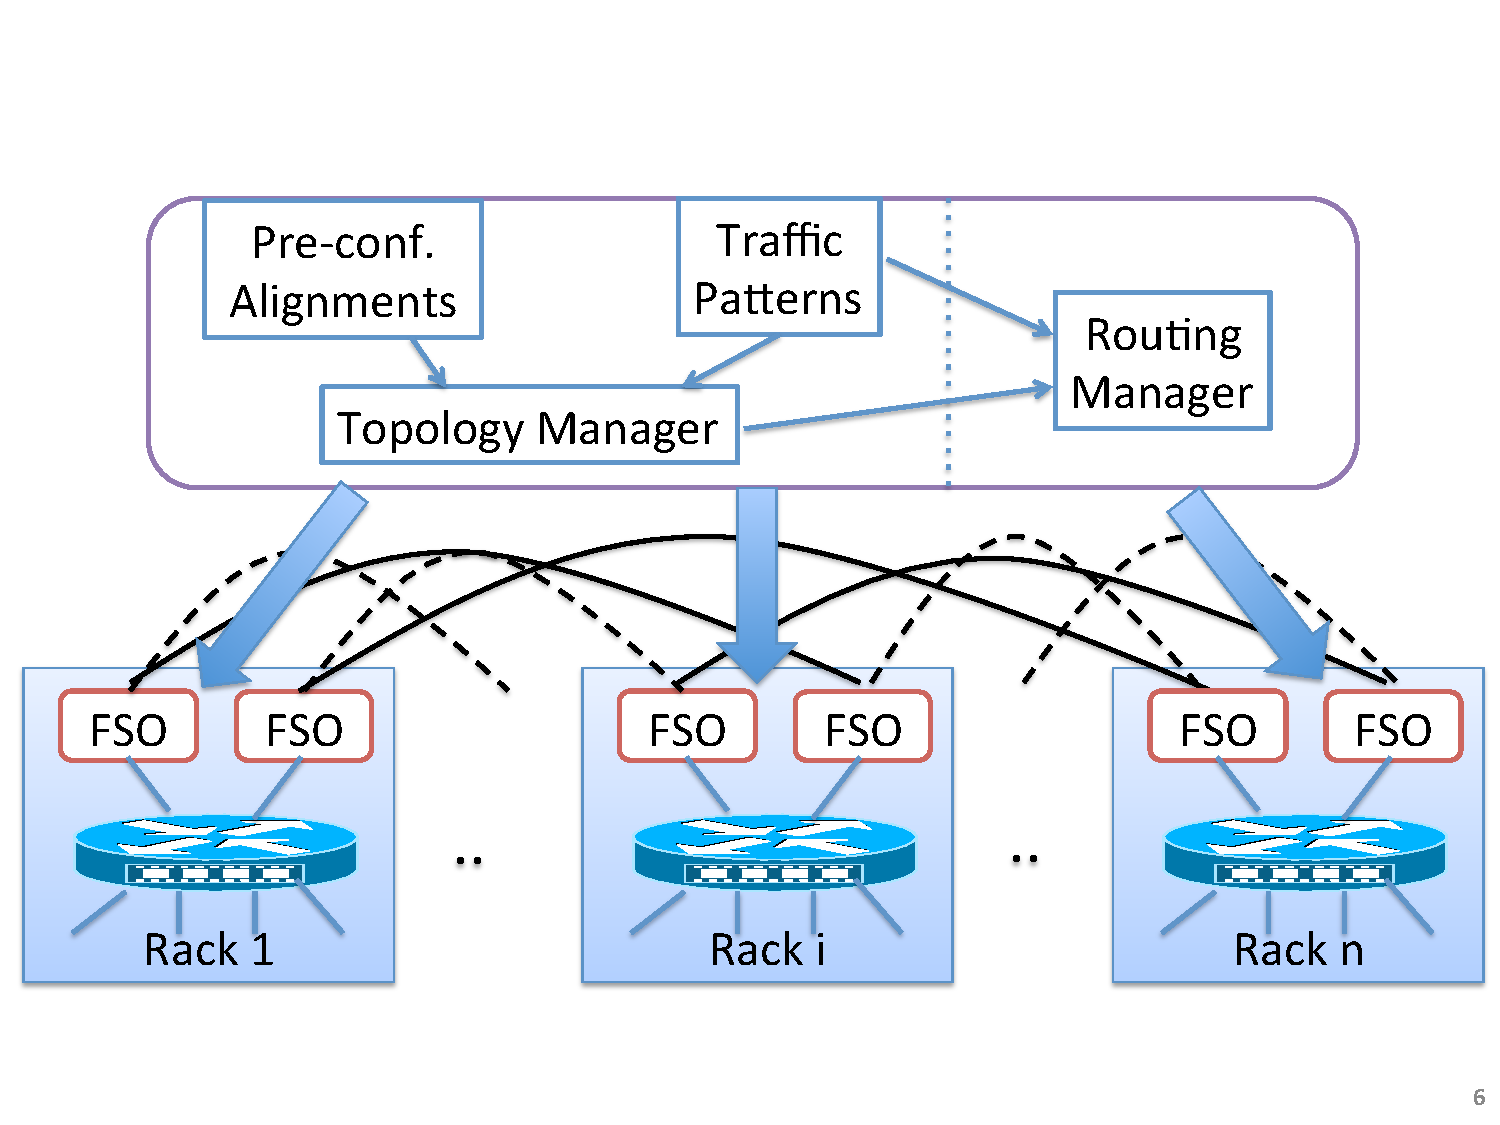
\includegraphics[width=200pt]{Figures/Architecture_New.pdf}
%\caption{\blue{System overview: The Topology Manager
%  decides the set of links to activate and the Routing Manager sets up
%  routes for end-to-end flows. At any instant, only one candidate link
%  per FSO is active (solid lines).} }
%\label{fig:arch}
%\end{figure}

\blue{One way to achieve a flexible architecture is to perform
  ``re-wiring'' of the ToR switches} on the fly using highly directed,
but steerable wireless links. Directivity is needed to
reduce/eliminate interference between neighbouring links. Directivity
in turn necessitates precise alignment between sender and receiver
pair.  We envision that these wireless links will connect the ToR
switches to form a fully flexible inter-rack fabric.\footnote{Note
  that we are not proposing a fully wireless data center as
  in~\cite{cornell}; our focus is on the `inter-rack' fabric
  only. Thus, the conventional wired rack architecture including the
  ToR switches remain.}  See Figure~\ref{fig:arch}.  The wireless
transceivers are to be placed on top of each rack.
%
We also envision a (centralized) {\em Topology Manager} that
dynamically reconfigures the inter-rack topology and a {\em Routing
  Manager} acts in concert with the Topology Manager to setup the
routing table entries for each ToR switch to route flows between
racks. 

\para{Choice of Wireless Technology: FSO Links.} We note that the
traditional radio-frequency technologies (e.g., 60GHz) suffer with
many shortcomings, especially in the context of realizing a
fully-flexible {\em all}-wireless inter-rack network. In particular,
RF links produce a large interference footprint due to a wide
beamwidth, even with 3D beamforming~\cite{3db}. Moreover,
beam-steering (needed to impart flexibility) technologies for RF links
are either slow and inaccurate~\cite{3db} or generate even larger
interference footprint~\cite{phased-arrays-rf}.
%
Lastly, the data rates of RF links fall off rapidly with
distance~\cite{3db}; higher transmit power can increase the range, but
also yields higher interference and energy usage, and is ultimately
limited by regulations.
%
\blue{To overcome the limitations of RF technology, we pursue a unique
  angle} -- use of free-space optics (FSO) to interconnect the ToR
switches. FSO communication~\cite{kedar} uses modulated visible or
infrared (IR) laser beams in the free space to implement a
communication link. Unlike traditional optical networks, the laser
beam in FSO is not enclosed in a glass fiber, but transmitted through
the air. There are two main benefits of FSO compared to traditional RF
technologies that make it a promising candidate for data centers:
%
\squishlist
\item[(a)] {\em Low Noise and Interference.}  Unlike RF links, FSO
  links do not suffer from multipath fading or \blue{EM}
  noises~\cite{}.  Moreover, FSO's beam divergence is many orders of
  magnitude narrower than RF (in the order of milliradians or less (1
  milliradian = $0.0573^\circ$). This reduces `interference footprint'
  to a negligible level.  Thus, FSO communications from multiple
  senders do not interfere, unless they are aligned to the same
  receiver (which is easy to avoid).

 \item[(b)]
  {\em High Data Rates over Long Ranges:}  Optical communications
inherently provide significantly higher data rates than any existing RF
technology owing to the use of much higher frequency and absence of
regulatory restrictions~\cite{kedar}. Coupled with much lower
attenuation of power over distance, FSO links are able to offer data
rates in the Gbps to Tbps regime at long distances (several kms) even
with modest transmit power (watts)~\cite{kedar}.
%
Commercially available FSO devices already offer data rates of
2.5~Gbps~\cite{fsona}, and demonstration systems even report data
rates in the order of Tbps~\cite{mustafa2013reintroducing} -- both for
long distance (in the order of km) links.
\squishend

\para{Key Challenges in FSO-based Inter-Rack Network.} While the key
characteristics of FSO technology facilitates design of an
all-wireless flexible inter-rack fabric, it also poses the following
challenges that must be addressed to make our vision a reality.

\begin{enumerate}
\item
{\em General Feasibility, and Precise and Fast Steering:}
  We must first demonstrate the feasibility of a small,
  cost-effective, and energy-efficient FSO device that is capable of
  delivering 10-100Gbps data rate. Second, we need to design and/or
  investigate mechanisms that will steer the laser beam with extreme
  precision (within microradians) and high speed (order of few tens of
  milliseconds). We address the above challenges in {\bf Section~\ref{sec:fso}}.

\item
{\em Pre-Configured Topology Design and Online Reconfiguration.}  Due
to the limited steerability of the \blue{considered} steering
mechanisms, we need to {\em pre-configure} the steering mechanism of
each FSO device (by pre-aligning or pre-orienting it) to a set/range
of other FSO devices. This pre-configuration determines the set of
fixed candidate links, from which the active links are chosen in
real-time (called {\em reconfiguration}) depending on the prevailing
traffic. We address the pre-configuration problem in {\bf
  Section~\ref{sec:top}}, and the reconfiguration problem along with
its related challenges in \bf{Section~\ref{sec:system}.}
\end{enumerate}
